\documentclass{standalone}

\usepackage{tikz}
\usetikzlibrary{fit}

\begin{document}

\providecommand{\XMHF}[2]{XMHF+}%

\newcommand{\Grid}[4]{
\foreach \i in {#1,...,#2}{
	\draw [color=cyan, opacity=0.5] (\i, #3) -- (\i, #4) node [above] {\i};
}
\foreach \i in {#3,...,#4}{
	\draw [color=cyan, opacity=0.5] (#2, \i) -- (#1, \i) node [left] {\i};
}
}%

\newcommand{\VulnInitDef}{
	\def\VulnInitA{0.75};
	\def\VulnInitB{0.5};
	\def\VulnInitC{0.75};
}%
\newcommand{\VulnInitCross}[4]{
	\draw[->, ultra thick] (#1, #3) -- (#2, #3 - \VulnInitA) node [pos=0.5, above, sloped] {#4};
}%
\newcommand{\VulnInitSelf}[4]{
	\draw[->, ultra thick] (#1, #2) .. controls (#1 + \VulnInitB, #2) and (#1 + \VulnInitB, #2 - \VulnInitA) .. (#1, #2 - \VulnInitA) node [pos=0.5, right, align=left] {#3};
}%

%

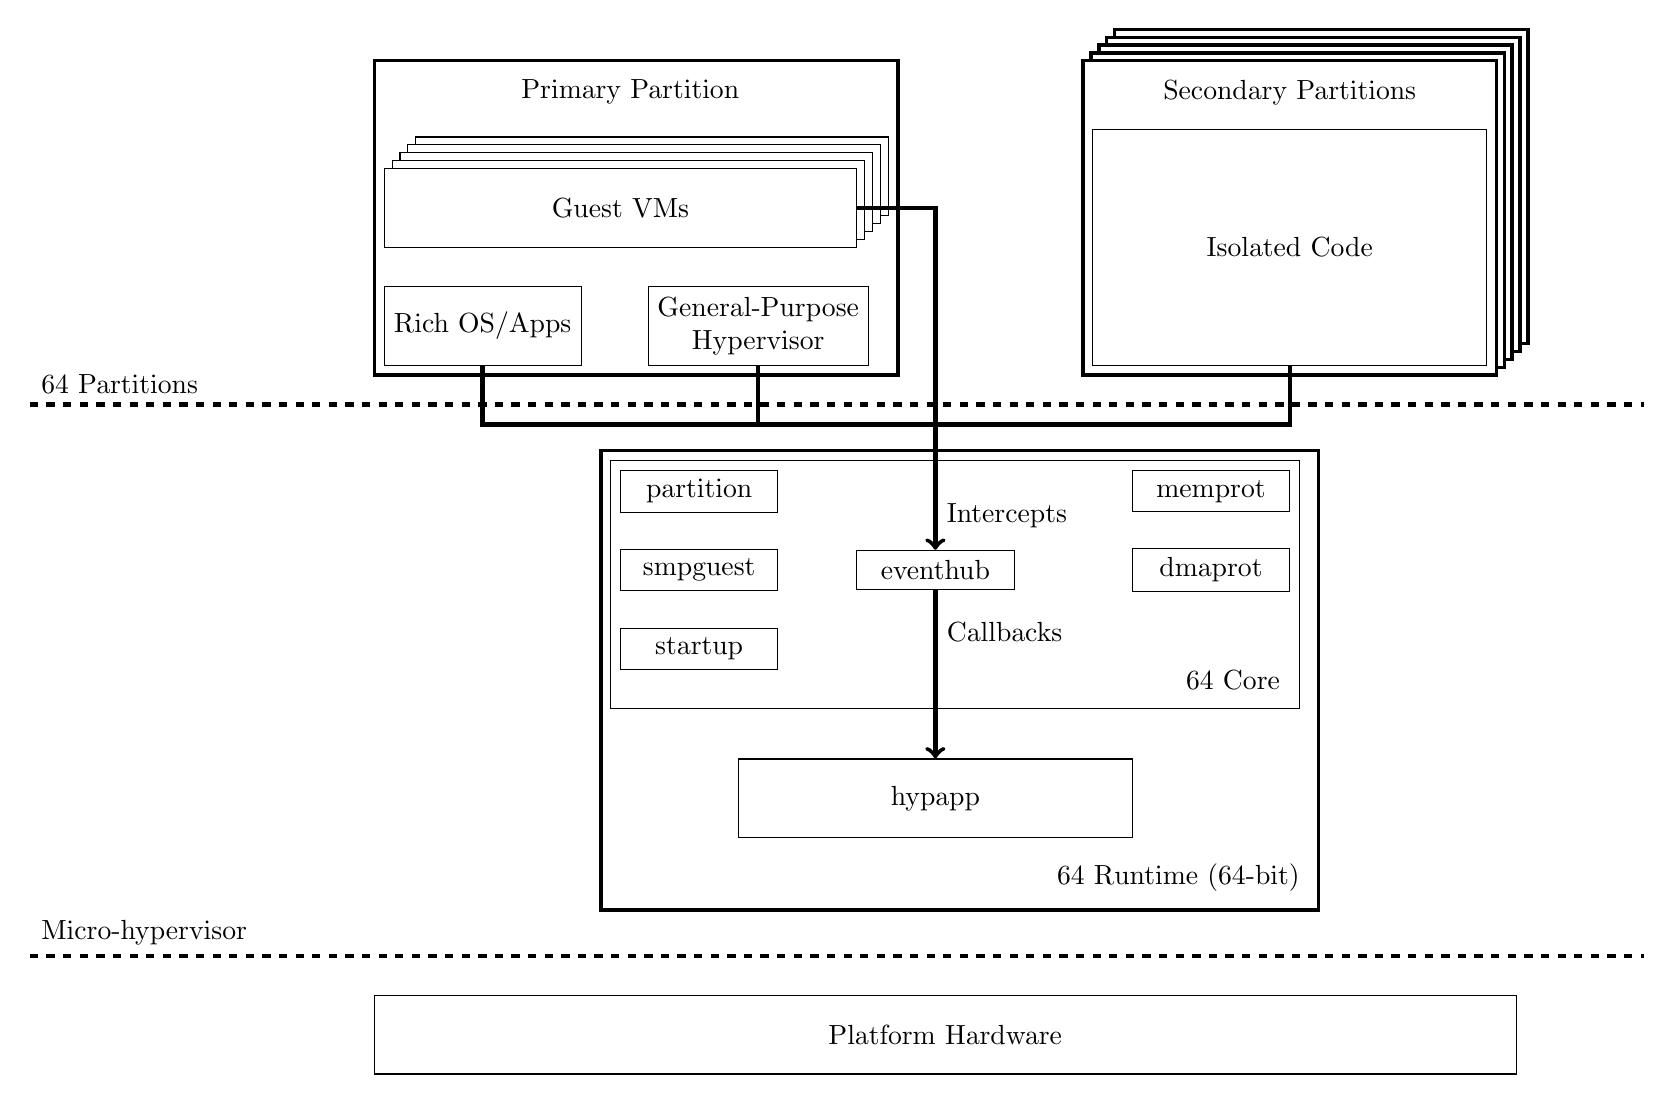
\begin{tikzpicture}

%\Grid{-9}{9}{0}{15}

\node (HW) at (1.125, 2) [rectangle, draw=black, minimum width=14.5cm, minimum height=1cm] {Platform Hardware};

\def\coreCompDy{0.1}
\node (hypapp) at (1, 5) [rectangle, draw=black, minimum width=5cm, minimum height=1cm] {hypapp};
\node (core-st) at (-2, 7-\coreCompDy) [rectangle, draw=black, minimum width=2cm, minimum height=0.5cm] {startup};
\node (core-pa) at (-2, 9-\coreCompDy) [rectangle, draw=black, minimum width=2cm, minimum height=0.5cm] {partition};
\node (core-sm) at (-2, 8-\coreCompDy) [rectangle, draw=black, minimum width=2cm, minimum height=0.5cm] {smpguest};
\node (core-dm) at (4.5, 8-\coreCompDy) [rectangle, draw=black, minimum width=2cm, minimum height=0.5cm] {dmaprot};
\node (core-me) at (4.5, 9-\coreCompDy) [rectangle, draw=black, minimum width=2cm, minimum height=0.5cm] {memprot};
\node (core-ev) at (1, 8-\coreCompDy) [rectangle, draw=black, minimum width=2cm, minimum height=0.5cm] {eventhub};
\node (core) at (5.5, 6.5) [left] {\XMHF64 Core};
\node (Core) [rectangle, draw=black, fit={(core-st) (core-pa) (core-sm) (core-dm) (core-me) (core-ev) (core)}] {};
\node (rt) at (5.75, 4) [left] {\XMHF64 Runtime (64-bit)};
\node (RT) [rectangle, draw=black, very thick, fit={(Core) (rt) (hypapp)}] {};

\def\lTwoVMsX{-3}
\def\lTwoVMsY{12.5}
\node (p1l1os) at (-4.75, 11) [rectangle, draw=black, minimum width=2.5cm, minimum height=1cm] {Rich OS/Apps};
\node (p1l1hv) at (-1.25, 11) [rectangle, draw=black, minimum width=2.5cm, minimum height=1cm, align=center] {General-Purpose \\ Hypervisor};
\newcommand{\DrawNested}[1]{
	\node (p1l2#1) at (\lTwoVMsX+0.#1, \lTwoVMsY+0.#1) [rectangle, draw=black, fill=white, minimum width=6cm, minimum height=1cm] {};
}
\foreach \x in {4,3,...,0}
	\DrawNested{\x}
\node (p1l2) at (\lTwoVMsX, \lTwoVMsY) [rectangle, draw=black, fill=white, minimum width=6cm, minimum height=1cm] {Guest VMs};
\node (p1) at (-2.875, 14.25) [below] {Primary Partition};
\node (P1) [rectangle, draw=black, very thick, fit={(p1l24) (p1l1os) (p1l1hv) (p1l2) (p1)}] {};
\def\partTwoX{5.5}
\def\partTwoY{12}
\newcommand{\DrawSecPart}[1]{
	\node (p2l1) at (\partTwoX+#1, \partTwoY+#1) [rectangle, minimum width=5cm, minimum height=3cm] {};
	\node (p2) at (\partTwoX+#1, 14.25+#1) [below] {};
	\node (P2) [rectangle, draw=black, very thick, fill=white, fit={(p2) (p2l1)}] {};
}
\foreach \x in {0.4,0.3,...,0}
	\DrawSecPart{\x};
\node (P2) [rectangle, draw=black, very thick, fit={(p2) (p2l1)}] {};
\node (p2l1) at (\partTwoX, \partTwoY) [rectangle, draw=black, minimum width=5cm, minimum height=3cm] {Isolated Code};
\node (p2) at (\partTwoX, 14.25) [below] {Secondary Partitions};

\draw[->, ultra thick] (core-ev) -- (hypapp) node [pos=0.25, right] {Callbacks};
\draw[ultra thick] (p1l1os) |- ++(3.5, -1.25);
\draw[ultra thick] (p1l1hv) |- ++(2.25, -1.25);
\draw[->, ultra thick] (p1l2.east) -| (core-ev) node [pos=0.95, right] {Intercepts};
\draw[ultra thick] (p2l1) |- +(-4.5, -2.25);

\draw[dashed, ultra thick] (-10.5, 3) -- ++(20.5, 0) node [pos=0, above right] {Micro-hypervisor};
\draw[dashed, ultra thick] (-10.5, 10) -- ++(20.5, 0) node [pos=0, above right] {\XMHF64 Partitions};

\end{tikzpicture}
\end{document}

